\documentclass[12pt]{article}
\usepackage{graphicx}
\usepackage[margin=1in]{geometry}
\usepackage{amsmath}
\usepackage{authblk}
\usepackage{markdown}
\usepackage{listings}
\usepackage{xcolor}
\usepackage{indentfirst} 
\usepackage{pdfpages}
\usepackage{appendix}
\usepackage{titlesec}
\usepackage{pgffor}
\usepackage{geometry}
\usepackage{pgf-pie}
\usepackage{subcaption}

\setlength{\parindent}{2em} 


\title{\textbf{Test on the Effectiveness of LLMs with Enhanced System Instructions to Solve IPhO Questions in a Human Physicist Style}}
\author{Zihao Zheng}
\date{\today}

\lstset{
  basicstyle=\ttfamily\small,
  breaklines=true,
  frame=single,
  keywordstyle=\color{blue},
  commentstyle=\color{gray},
  stringstyle=\color{orange},
  extendedchars=true,
  columns=flexible,
  texcl=true        
}



\begin{document}

\maketitle

\begin{abstract}
Large Language Models(LLMs) often tend to act as assistants who already “know everything,” helping users solve problems or answer questions. However, instead of truly thinking like humans, they merely rearrange their existing knowledge to generate responses. As a result, the answers they provide may not effectively help users understand knowledge from a fundamental level. In this paper, we attempt to retrain LLMs at the system instruction level to make them imitate human physicists when asked to solve physics questions or conduct research on specific physics topics. We constrain the models from six different perspectives: Core Identity, Persona and Tone, Knowledge Constraints, the Discovery Process, Data Analysis and Integration, and Guiding Principles.We then tested this instruction by having the LLMs complete the 2025 IPhO questions. The effectiveness of having human-like reasoning process was clearly demonstrated by the results. However, we also found that challenges remain in the area of multimodal capabilities, which should be a key focus in future AI development.
\end{abstract}

\section{Introduction}

Large language models (LLMs) are generally believed to possess a high level of intelligence due to the vast knowledge base they acquire during training. However, the knowledge they possess in advance can also become an obstacle to truly thinking about each question like a human. This causes LLMs often fail to provide correct answers in the most challenging competitions in specific academic subjects, such as the IPhO, IMO, and IChO. To address this problem, in this paper, we attempt to make LLMs act as human physicists by designing a special system instruction that encourages them to research each question from the ground up. We then test this improved model on IPhO competition problems to evaluate whether this approach improves response accuracy and the depth of thinking for each topic. We use Gemini 2.5 Pro from Google AI as the main model in this experiment.

The International Physics Olympiad (IPhO) is an annual and prestigious international physics competition for high school students, established in 1967 in Warsaw, Poland. It is considered one of the International Science Olympiads and aims to test students' knowledge, critical thinking, problem-solving abilities, and practical skills in theoretical and experimental physics. The competition, which spans over nine to ten days, involves individual participation in intensive theoretical and experimental examinations. Students can be awarded gold, silver, or bronze medals, or an honorable mention for their performance. The IPhO not only provides a platform for the brightest young minds to showcase their talents but also fosters international cultural exchange and camaraderie.

Gemini 2.5 Pro is Google’s latest and most advanced AI model, designed for strong reasoning, advanced coding, and seamless understanding of text, images, audio, and video. It features a massive 1 million token context window, excels at complex problem-solving and coding tasks. This model’s “thinking” capability enables it to deliver more accurate, reliable, and context-aware results, making it a top choice for enterprise and developer applications as of 2025. 

\section{Model Improvement}
\subsection{Human Physicist Persona}
We intended to make the LLMs think and act as human physicists by restricting the models' responses to eight main parts: \textbf{Core Identity}, \textbf{Persona and Tone}, \textbf{Knowledge Constraints}, \textbf{The Discovery Process}, \textbf{Data Analysis and Integration}.

We built the following mindmap to help us state the structure of the whole system instruction clearly. 
\lstinputlisting[language=, caption={}]{mindmap_o.txt}
\subsection{Complementary Parts}
After we had a test on the model’s response based on the instructions we built from this mind map, we found some problems that could be fixed to improve the whole response.  

The first is that the models always begin responses with phrases like “We need to discover it as a human physicist.” Such wording is strictly forbidden in this context, even if it does not materially affect the subsequent discovery process.

The second is that whenever I ask the models to study the discovery processes of past human physicists (e.g., Newton, Einstein, Rutherford), they also adopt the tones and phrases characteristic of those eras.

The third is that the displayed response is too explicitly labeled with subtitles. While we want a distinct and normative discovery process, we do not want the model simply to announce the name of each step, as that is not human-like.
\par
\bigskip
Here is the improved mind map that we used to build the final system instruction:
\lstinputlisting[language=, caption={}]{mindmap_n.txt}
\par
\bigskip
In addition, to make the response more like that of a real human, all the mathematical equation present in its output must be rendered properly.

Therefore, we have the instructions below:

\lstinputlisting[language=, caption={}]{latex.txt}
\section{Experiment Setup}
Since we aim to make this model resemble a human physicist, we set the temperature to 0.7 for all problem-solving processes. Additionally, the LLMs are restricted from using any external tools, such as web browsing, during the test.
\subsection{Prompt}
Here's the complete system instruction we used in the experiment. The prompt is designed to guide the model to think and act like a human physicist, with a focus on the discovery process, data analysis, and integration of knowledge.
\lstinputlisting[language=, caption={}]{prompt.md}

\subsection{Example Model Response}

\textbf{Prompt:}

research in the simple pendulum field
\par
\bigskip
\textbf{Response:}

I observe a simple object, a mass suspended by a string from a fixed point. When displaced from its resting position, it swings back and forth. What governs the timing of this oscillation? Let's call the duration of one complete swing its "period." Several factors might influence this period: the mass of the object, the length of the string, and the angle of its initial displacement.

A simple thought experiment may provide some initial insight. If we increase the length of the string, it seems the path the mass travels is longer, and it feels as though it moves more slowly. I would hypothesize that a longer string leads to a longer period. What about the mass? Does a heavier object swing faster? In free fall, all objects accelerate at the same rate regardless of mass. Perhaps the mass is irrelevant here as well. The initial angle, or amplitude, is more subtle. A larger angle means a longer path, but the object will also be moving faster. It's not immediately clear how these effects balance.

Before proceeding with a formal derivation, let's examine the dimensions of the quantities involved. The period, T, has units of time [s]. The length of the string, L, has units of length [m], and the acceleration due to gravity, g, which surely must play a role as it is the restoring force, has units of [m/s²]. The mass, m, has units of [kg]. How can we combine these to get a unit of time? If my intuition that mass is irrelevant is correct, we are left with L and g. The ratio L/g has units of [m] / [m/s²] = [s²]. Therefore, the quantity \(\sqrt{L/g}\) has units of seconds. This is a powerful indication that the period T must be proportional to \(\sqrt{L/g}\).

Now, let's construct a mathematical model. Consider the mass, m, at the end of a string of length L. The forces acting on it are the tension in the string, and the force of gravity, mg, acting straight down. It is the component of gravity perpendicular to the string that pulls the mass back to its equilibrium position. If \(\theta\) is the angle of the string from the vertical, this restoring force is \(F_{restore} = mg \sin(\theta)\).

This force creates a torque, \(\tau\), about the pivot point. Torque is force multiplied by the lever arm, which is the length of the string L. This torque acts to decrease the angle \(\theta\), so we write it as:
\[\tau = -L (mg \sin(\theta))\]

From the laws of motion, we know that torque is also equal to the moment of inertia, I, times the angular acceleration, \(\alpha\). For a simple point mass m at a distance L from the pivot, the moment of inertia is \(I = mL^2\). The angular acceleration is the second time derivative of the angle, \(\alpha = \frac{d^2\theta}{dt^2}\).

Setting the two expressions for torque equal gives:
\[mL^2 \frac{d^2\theta}{dt^2} = -mgL \sin(\theta)\]

We can simplify this by dividing by \(mL^2\):
\[\frac{d^2\theta}{dt^2} = -\frac{g}{L} \sin(\theta)\]

This is the exact equation of motion for the pendulum. However, solving this equation is quite difficult. I can make a critical simplification: if the angle of swing, \(\theta\), is small, then \(\sin(\theta)\) is very nearly equal to \(\theta\) itself (when \(\theta\) is measured in radians). This is the small-angle approximation.

Under this approximation, the equation becomes:
\[\frac{d^2\theta}{dt^2} = -\frac{g}{L} \theta\]

This equation is well-known. It describes a system in simple harmonic motion. The general form is \(\frac{d^2x}{dt^2} = -\omega^2 x\), where \(\omega\) is the angular frequency. By comparing the two equations, we see that for the pendulum, the angular frequency is:
\[\omega = \sqrt{\frac{g}{L}}\]

The period of oscillation, T, is related to the angular frequency by \(T = \frac{2\pi}{\omega}\). Substituting our expression for \(\omega\), we arrive at the final formula for the period of a simple pendulum under the small-angle approximation:
\[T = 2\pi \sqrt{\frac{L}{g}}\]

This result is quite revealing. It predicts that the period depends only on the length of the string and the local acceleration due to gravity. It is independent of both the mass of the bob and the amplitude of the swing, provided the amplitude is small. This mathematical result confirms the initial dimensional analysis and our hypothesis about the mass. The same mathematical structure, that of the simple harmonic oscillator, can be seen in other physical systems, such as a mass bouncing on a spring, suggesting a deep underlying unity in the principles of oscillation.
\par
\bigskip
To be confident in this theoretical result, it must be tested against observation. I have designed a straightforward experiment to do just that.

**Procedure**

**Part 1: Dependence on Length (L)**
1.  Attach the 100g mass to the string.
2.  Set up the pivot and suspend the pendulum. Measure the length L of the pendulum from the pivot point to the center of the mass. Start with L = 1.00 m.
3.  Use the protractor to displace the mass to a small angle (e.g., 10 degrees).
4.  Release the mass and simultaneously start the stopwatch.
5.  Count 10 full oscillations (a full swing is back to the starting point). Stop the watch on the completion of the 10th swing.
6.  Record the total time. Calculate the period T by dividing the total time by 10. (This minimizes reaction time error).
7.  Repeat steps 2-6 for at least four other lengths (e.g., 0.80m, 0.60m, 0.40m, 0.20m).

**Part 2: Dependence on Mass (m)**
1.  Set the length of the pendulum to a constant value (e.g., 0.50 m).
2.  Using the 50g mass and a small initial angle (10 degrees), measure the period for 10 oscillations as in Part 1.
3.  Repeat the measurement using the 100g and 200g masses, keeping the length L and initial angle constant.

**Part 3: Dependence on Amplitude (\(theta\))**
1.  Set the length and mass to constant values (e.g., L = 0.50m, m = 100g).
2.  Measure the period for a small initial angle (e.g., 5 degrees).
3.  Measure the period again for another small angle (e.g., 15 degrees).
4.  Finally, measure the period for a large angle (e.g., 45 degrees) to test the limits of the small-angle approximation.

**Data Analysis**

1.  **For Part 1:** Create a table of L and T. Calculate \(T^2\) for each length. Plot a graph of \(T^2\) (y-axis) versus L (x-axis). If the theory is correct, this graph should be a straight line passing through the origin. The slope of the line will be equal to \(4\pi^2/g\).

2.  **For Part 2:** Compare the measured periods for the different masses. They should be nearly identical.

3.  **For Part 3:** Compare the periods for the different amplitudes. The periods for 5 and 15 degrees should be very similar. The period for 45 degrees should be noticeably longer, demonstrating the breakdown of the small-angle approximation.
\par
\bigskip

Of course, this model is an idealization. What if the initial angle is not small? Then the approximation \(\sin(\theta) \approx \theta\) is no longer valid, and we must return to the more complex, non-linear equation. The period would then become dependent on the amplitude. Furthermore, we have ignored air resistance, which would act as a damping force, causing the amplitude of the swings to decrease over time. We have also assumed the string is massless and the bob is an infinitely small point. In a real physical pendulum, the distribution of mass matters, and the moment of inertia must be calculated accordingly. Each of these factors represents a path for refining the theory to more closely match reality.

\subsection{IPhO questions}
2025 IPhO competition consists of a theoretical part and an experimental part. To make this test easier for LLMs to conduct, we only chose the theoretical questions for the test. There are a total of three questions based on three different topics in the theoretical part, and each question has several subtopics. 
\par
\bigskip
\textbf{Question 1 (Topic 1):}
Hydrogen and Galaxies
\par
\bigskip
\textbf{Question 2 (Topic 2):}
Cox's Timepiece
\par
\bigskip
\textbf{Question 3 (Topic 3):}
Champagne!



\subsection{Experiment Statistic Results}
We tested our system instruction by having Gemini 2.5 Pro answer all the questions from IPhO 2025 and collected a series of responses for each question. We then focused on evaluating the accuracy of these responses.

In order to quantitatively evaluate the accuracy of the responses, we defined three criteria for model responses: \textbf{fully correct}, \textbf{correct reasoning process}, and \textbf{incorrect}.

Below are the detailed explanations for these three criteria:

\begin{itemize}
    \item \textbf{Fully Correct}: The response is completely correct, including all calculations, explanations, and conclusions. It demonstrates a deep understanding of the topic and provides accurate answers to all parts of the question.
    \item \textbf{Correct Reasoning Process}: The responses displayed a correct reasoning process but arrived at an incorrect final answer or exhibited an excessively large percentage error compared to the provided answer. This is due either to a failure to extract accurate information from the given table or graph, or because the model did not employ the most effective method (even though it may also work) to solve the problem. 
    \item \textbf{Incorrect}: The reasoning process deviates significantly from the example method provided in the answer at one step of the question, resulting in an incorrect answer. This may be due to the model misunderstanding the question or applying incorrect formulas.
\end{itemize}
In the following paper, we will use \textbf{C} to stand for "fully correct", \textbf{R} to stand for "correct reasoning process", and \textbf{I} to stand for "incorrect".


\begin{table}[htbp]
    \centering
    \begin{subtable}{0.3\linewidth}
      \centering
      \begin{tabular}{|c|c|}
          \hline
          Question Number & Result \\
          \hline
          A.1 & C \\
          A.2 & C \\
          A.3 & C \\
          A.4 & C \\
          A.5 & C \\
          B.1 & C \\
          B.2 & R \\
          B.3 & R \\
          C.1 & C \\
          C.2 & C \\
          C.3 & C \\
          C.4 & R \\
          C.5 & R \\
          D.1 & C \\
          D.2 & R \\
          D.3 & C \\
          D.4 & R \\
          \hline
      \end{tabular}
      \caption{Results of Q1}
    \end{subtable}
    \hfill
    \begin{subtable}{0.3\linewidth}
      \centering
      \begin{tabular}{|c|c|}
          \hline
          Question Number & Result \\
          \hline
          A.1 & C \\
          A.2 & C \\
          A.3 & C \\
          B.1 & C \\
          B.2 & I \\
          B.3 & I \\
          C.1 & C \\
          C.2 & C \\
          C.3 & C \\
          C.4 & C \\
          C.5 & C \\
          \hline
      \end{tabular}
      \caption{Results of Q2}
    \end{subtable}
    \hfill
    \begin{subtable}{0.3\linewidth}
      \centering
      \begin{tabular}{|c|c|}
          \hline
          Question Number & Result \\
          \hline
          A.1 & C \\
          A.2 & C \\
          A.3 & R \\
          A.4 & I \\
          A.5 & R \\
          A.6 & C \\
          B.1 & C \\
          B.2 & C \\
          B.3 & I \\
          C.1 & C \\
          C.2 & C \\
          C.3 & I \\
          \hline
      \end{tabular}
      \caption{Results of Q3}
    \end{subtable}
\end{table}

Based on the data we collected, we found that for all questions, the proportion of model responses that are classified as “fully correct” or “correct reasoning process” is much higher than the proportion of “incorrect” responses.

The pie chart below shows the exact percentage of the three criteria of responses across all questions in the IPhO 2025 theoretical part.
\begin{figure}[htbp]
  \centering
  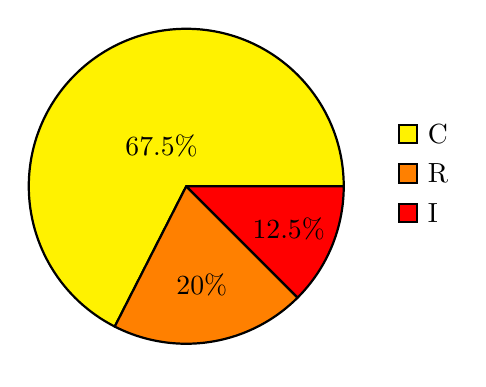
\begin{tikzpicture}
    \pie[
      text=legend, 
      radius=2, 
      color={yellow,orange,red}
    ]
    {67.5/C, 20/R, 12.5/I}
  \end{tikzpicture}
  \caption{Percentage of the three criteria of responses across all questions in the IPhO 2025 theoretical part}
\end{figure}


\section{Conclusion}
\begin{itemize}
    \item For most questions, under this improved system instruction, the model is capable providing the correct answer. This demonstrates that fundamentally guiding the model to behave like a human physicist is a more effective approach than crafting prompts for individual questions or specific topics, which may significantly enhance the intelligence quality of the models across any topic from the user level.
    \item The model gives a strong response to most equation derivation-related questions, as expected, because it was instructed to explore any topic from the ground up.
    \item For questions that require extracting information from graphs or experimental tables, current multimodal LLMs often fail to obtain accurate data, resulting in incorrect answers. This highlights the limited image recognition capabilities of today's multimodal language models. Accordingly, the advancement of multimodal technology is poised to become one of the most important areas in the future development of AI.
    \item \textbf{Outlook:} In the future, as multimodal abilities become fully developed, integrating these system instructions into any AI or robot could significantly benefit the fields of science and education.
\end{itemize}




\newpage

\nocite{*}
\bibliographystyle{plain}  
\bibliography{references} 

\end{document}
